% ============================================================
% 单栏版 — 流感知 GNN 的 QoS 约束路由（中文正文，IEEE 数字制引用）
% 编译: xelatex main_onecol.tex; bibtex main_onecol; xelatex×2
% 与 main.tex 共用 sections/ 与 related_work.bib，仅版式改为单栏
% ============================================================
\documentclass[lettersize,journal]{IEEEtran}

\usepackage{ctex}              % 中文支持 (xelatex)
\usepackage{amsmath,amssymb}
\usepackage{graphicx}
\graphicspath{{figures/}}
\usepackage{booktabs}
\usepackage{array}
\usepackage{multirow}
\usepackage{url}
\usepackage{xcolor}
\usepackage[ruled,linesnumbered]{algorithm2e}  % 训练流程伪代码
%\usepackage{geometry}    % 单栏更宽，留合理边距

\title{QoS-FiLM: Flow-Intent-Conditioned GNNs for Online QoS Routing}

\begin{document}
\maketitle

\begin{abstract}
Modern backbone networks carry heterogeneous traffic where small flows demand strict latency guarantees and large flows seek high throughput. Existing online routing heuristics are myopic because they cannot foresee future arrivals; prevailing learning-based methods generate a single topology embedding for all flows regardless of their QoS intent, which limits their ability to differentiate routing under mixed services. We present QoS-FiLM, an encoder that conditions each message passing layer of a graph neural network (GNN) on the QoS intent of individual flows via Feature-wise Linear Modulation (FiLM). Identical substrate graphs are thereby embedded differently for heterogeneous flows. We formulate online per flow routing as a stochastic Markov decision process and train the policy with proximal policy optimization (PPO). Experiments on GEANT, NOBEL-EU, and ABILENE topologies show that QoS-FiLM outperforms several baselines in cumulative utility, bandwidth satisfaction ratio, and end to end latency. \textcolor{red}{这句结论得改一下，不完整，没有学习型方法}On GEANT, the mean reward improves by 0.121 over the strongest heuristic, the bandwidth score reaches 0.759, and the average delay drops to 112.9 ms. Ablation studies confirm that FiLM conditioning is essential and that it interacts strongly with the attention operator. Interpretability analysis verify that the encoder is highly sensitive to QoS intent, while the policy causally divides routing decisions based on flow type.
\end{abstract}

\begin{IEEEkeywords}
online routing, graph neural networks, QoS differentiation, featurewise linear modulation, deep reinforcement learning
\end{IEEEkeywords}

% ===== 章节（与 main.tex 共用同一批 section 文件） =====
\section{Introduction}
\label{sec:intro}

互联网流量的异构化已成为骨干网面临的核心挑战。同一基础设施需同时承载交互式视频、远程控制、分布式 AI 训练与批量备份等业务，这些业务对带宽、时延、丢包等 QoS 维度的偏好差异巨大，形成了``老鼠流''（带宽小、QoS 要求严苛）与``大象流''（带宽巨大、容忍尽力而为）共存的混合特征\cite{CISCO2023_GlobalTraffic}。这种差异化需求使得传统无差异化的路由策略——无论是基于最短跳数的OSPF 还是等价多路径的 ECMP——在资源利用与 QoS 保障之间顾此失彼。

问题的本质困难在于在线因果耦合：流逐条到达且未来不可见，智能体为第$t$ 条流选路时无法预见 $t+1,\dots,W$ 的后续需求\cite{Wang1996_QoSRouting}。若允许离线处理整条流序列，选路可建模为整数规划求得全局最优；但在线约束迫使决策必须在信息不完备下做出，导致先到流与后到流竞争共享链路容量。贪心启发式（如 CSPF）虽每步局部最优，却常将早期到达的老鼠流优先分配至资源充裕的最优路径，耗尽后续大象流所需的链路容量，这正是短视启发式策略的经典困境\cite{Fortz2000_TrafficEngineering}。最优策略必须非短视地在需求分布的期望意义下预留容量、跨流权衡，并将序列末尾的累积效用回溯归因到早先各步——这种``未来不可见下的序贯决策与长程信用分配''的结构，天然适合用强化学习（RL）求解。

近年来，深度强化学习（DRL）与图神经网络（GNN）的结合为在线路由带来了新的可能：DRL 提供了非短视的序贯决策能力\cite{Sun2022_ScalableRouting_TON,He2024_RoutingOptimization_TMC}，GNN 提供了对网络拓扑的显式编码能力\cite{Rusek2020_JSAC_RouteNet, FerriolGalmes_2023_RouteNetFermi}。然而，现有方法存在两个深层局限：其一，DRL 路由策略通常为所有流优化单一全局目标，无法在混合业务下实现差异化服务；其二，GNN 方法为所有流学习统一的拓扑嵌入，无法根据逐流的 QoS 特征对同一拓扑进行差异化感知，即``同图同嵌入''问题。

要打破``同图同嵌入''的同质化限制，需要使网络编码器具备流条件化能力，即根据每条流的个体 QoS 特征动态调整其拓扑感知。条件化神经网络（conditional neural networks）为此提供了核心工具。Perez 等人提出的 FiLM（Feature-wise Linear Modulation）通过仿射变换将辅助信息注入网络各层\cite{Perez2018_FiLM}，Brockschmidt 等人将其拓展至图领域（GNN-FiLM），以目标节点表示调制消息传递\cite{Brockschmidt2020_GNNFiLM}。但在在线路由场景中，真正需要条件化的并非目标节点，而是逐流的 QoS 意图：同一张拓扑在面对老鼠流与大象流时，其消息传递过程应当被重塑为两种截然不同的拓扑感知。现有文献尚未将 FiLM 条件化机制引入逐流在线路由场景，使得混合业务下的差异化拓扑感知与策略学习成为开放问题。

针对上述差距，本文提出流感知 FiLM-GNN 编码器，核心思想是：通过 FiLM 将每条流的 QoS 意图向量注入 GNN 的每一层消息传递，使同一张物理拓扑在不同意图下被编码为差异化的节点嵌入。进而，我们将在线混合业务选路形式化为马尔可夫决策过程（MDP），以近端策略优化（PPO）训练非短视选路策略。本文的主要贡献如下：
\begin{itemize}
    \item \textbf{面向混合业务在线路由的流感知图强化学习架构：}
    该架构由流条件化图编码器、路径感知打分器与独立价值网络三部分构成，通过近端策略优化实现端到端训练，解决了同一拓扑需对不同QoS意图流产生差异化路由决策的核心矛盾。

    \item \textbf{逐流QoS意图驱动的FiLM条件化机制与网络设计：}
    以逐流意图向量生成图神经网络各层的仿射调制参数，使消息传递过程成为流感知的；配套设计了基于LSTM的路径嵌入池化、意图-路径联合打分及意图条件化注意力图池化等关键模块，实现了从拓扑编码到路径选择的完整流条件化决策链路。

    \item \textbf{双空间可解释性实验验证：}
    实验表明所提架构在累积效用、带宽满足比和端到端时延上显著优于经典基线；进一步通过表示空间（隐藏特征分离度）与决策空间（路径选择分化）的双重分析证实：仅改变QoS意图即可在相同拓扑、相同源宿节点对下触发差异化路由决策，从机理层面验证了FiLM条件化的必要性。
\end{itemize}

\section{Related Work}
\label{sec:related}

本节从传统 QoS 路由、深度强化学习驱动的路由、图神经网络的网络建模能力、以及图网络条件化机制四个维度，综述与本问题密切相关的近期研究，并在末段明确本文定位。

\subsection{传统 QoS 路由与流量工程}

OSPF、ECMP、CSPF 等经典协议基于静态链路权重做逐跳转发，在混合业务场景下缺乏差异化服务能力。Wang 与 Crowcroft 奠定了 QoS 路由的约束优化框架\cite{Wang1996_QoSRouting}；Fortz 与 Thorup 揭示了基于权重优化的流量工程在动态需求下的局限性\cite{Fortz2000_TrafficEngineering}。Brundiers 等人研究了 Segment Routing 中环路对流量工程的增益，展示了灵活路径控制在动态负载均衡中的潜力\cite{Brundiers2021_Loops_SR_TE}，并进一步提出了中点优化方法以实现更细粒度的流量工程控制\cite{Brundiers2022_Midpoint_SR_INFOCOM}。这些方法的共同缺陷在于短视性:每步决策独立优化，无法在网络全局与序列长远视角下为异构流预留资源。当老鼠流与大象流共享链路时，静态策略往往在保障低时延与追求高吞吐之间顾此失彼。

\subsection{深度强化学习驱动的网络路由}

为突破固定规则的局限，研究者将 DRL 引入路由决策。Liu 等人针对多类型业务需求提出了 DRL-OR，在在线路由中实现了对异构服务的差异化处理\cite{Liu2021_DRLOr_INFOCOM}。Casas-Velasco 等人提出了 DRSIR，以深度 Q 学习在 SDN 中实现智能路由决策\cite{CasasVelasco2021_DRSIR_TNSM}。Chen 等人提出了基于多智能体元强化学习的自适应多路径路由优化框架\cite{Chen2022_MultiagentMeta_TNNLS}。Suzuki 等人提出了多智能体深度强化学习方法，在多云边缘网络中联合优化计算卸载与路由决策，验证了多智能体协作在动态网络环境中的自适应能力\cite{Suzuki2023_MADRL_Routing_TNSM}。Sanchez 等人提出了 DQS，以 QoS 驱动的深度强化学习实现 SDN 中的路由优化\cite{Sanchez2024_DQS_JPDC}。然而，上述方法存在两个共性局限：其一，策略网络大多以全连接层或简单嵌入编码网络状态，缺乏对拓扑结构的显式建模能力，泛化性受限；其二，它们通常为所有流优化单一的全局目标（如最小化最大链路利用率或平均时延），未将逐流 QoS 意图作为条件信号嵌入策略网络，无法在混合业务下实现差异化路由。

\subsection{图神经网络的网络建模与路由优化}

图神经网络（GNN）为编码网络拓扑提供了自然工具。Rusek 等人利用消息传递神经网络建模链路时延与丢包，开创了 RouteNet 系列工作\cite{Rusek2020_JSAC_RouteNet}。Ferriol-Galm\'{e}s 等人进一步提出 RouteNet-Fermi，通过增强的 GNN 架构实现大规模网络性能预测与优化\cite{FerriolGalmes_2023_RouteNetFermi}。Huang 等人提出了xNet，通过学习时序状态转移函数实现细粒度流级 QoS 预测\cite{Huang2024_ToN_xNetModeling}。Munikoti 等人系统综述了深度强化学习与图神经网络结合的挑战与机遇，揭示了现有方法在复杂网络优化中的瓶颈\cite{Munikoti2024_DRL_GNN_TNNLS}。Almasan 等人探索了 GNN 与 DRL 在路由优化中的联合应用，验证了图结构感知对策略质量的提升\cite{Almasan2022_RLmeetsGNN}。Bern\'{a}rdez 等人提出了 MAGNNETO，以基于 GNN 的多智能体系统在流量工程优化中实现了分布式决策与快速响应\cite{Bernardez2023_MAGNNETO_TCCN}。Bhuvanasi 等人利用 GNN 与多智能体 DRL 实现了对拓扑变化的弹性路由\cite{Bhuvanasi2023_ResilientRouting_TNSM}。Yang 等人将图卷积网络与 DRL 结合，在时间敏感网络中联合优化路由与调度\cite{Yang2022_GCN_RL_IoTJ}。Dong 等人提出了基于 GCN 的多任务深度强化学习方法，在网络切片与路由的联合优化中验证了图感知策略的有效性\cite{Dong2022_GCN_Slicing_Routing_TCCN}。然而，现有 GNN 方法存在结构性的表示同质化问题：它们要么聚焦于聚合流量下的离线性能建模（如 RouteNet），学习``一张图、一种全局嵌入''；要么在在线决策中为所有流生成统一的拓扑表示（如 GNN+DRL 方法）。这意味着，当老鼠流与大象流先后到达时，系统看到的是同一张图的同一个嵌入，无法根据逐流的 QoS 特征对同一拓扑进行差异化感知，更无法据此做出差异化的路由决策。

\subsection{图神经网络的条件化机制}

为使网络表示能够根据外部条件动态调整，研究者提出了多种条件化机制。Perez 等人提出的 FiLM（Feature-wise Linear Modulation）通过仿射变换将辅助信息注入神经网络各层 \cite{Perez2018_FiLM}；Brockschmidt 等人将其拓展至图领域，提出 GNN-FiLM，以目标节点表示调制消息传递过程 \cite{Brockschmidt2020_GNNFiLM}。在异构图学习领域，Hu 等人提出的 Heterogeneous Graph Transformer 通过节点类型条件化注意力来区分不同语义关系 \cite{Hu2020_HGT}；Brody 等人提出的 GATv2 以动态注意力机制实现了边级条件化权重计算 \cite{Brody2022_GATv2}。然而，上述条件化机制主要服务于节点分类、分子生成或静态图表示学习任务，其调制信号来源于图内结构（目标节点、边类型、节点类别等），而非逐流的外部 QoS 意图。在在线路由场景中，真正需要条件化的并非图内节点属性，而是到达流的 QoS 特征：同一张拓扑在面对老鼠流与大象流时，应当产生截然不同的嵌入与决策。现有文献尚未将 FiLM 条件化机制引入逐流在线路由场景，使得混合业务下的差异化拓扑感知与策略学习成为开放问题。


综上，现有工作存在明确缺口：（1）传统方法短视且无法处理混合 QoS；（2）DRL 方法缺乏拓扑显式建模；（3）GNN 方法假设同质流量；（4）条件化 GNN 尚未引入逐流在线路由。本文填补上述差距，提出流感知 FiLM-GNN 架构，以逐流 QoS 意图作为外部条件信号，通过 FiLM 重塑 GNN 的每层消息传递，使同一张物理拓扑在异构业务流下被编码为差异化的策略输入，进而以 PPO 训练非短视的在线选路策略。
\section{问题定义}
\label{sec:problem}

本节定义 QoS 约束下的逐流选路问题，约定全文使用的数学符号，给出效用函数与优化目标，并在章末论证为何该问题需要用强化学习求解。

\subsection{网络与流量模型}
\label{sec:problem:model}

考虑一个有向网络 $G=(V,E)$，节点集 $V$、链路集 $E$。每条链路 $e\in E$ 具有时延 $d_e$ 与带宽容量 $c_e$；记其在某一时刻的剩余带宽为 $b_e^{\text{res}}\in[0,c_e]$，初始时 $b_e^{\text{res}}=c_e$。

流量以\emph{序列}（episode）为单位在线到达：一个序列内有 $W$ 条流逐条到达，智能体即时为每条流选路、且无法预见后续到达的流。每条流一旦被指派路径，便在本序列内持续占用其带宽——这是在线选路中的”永久连接 / 无限保持时间”假设，本文不建模流的离去。序列结束后容量重置、开始新的一批到达。

第 $t$ 条流由四元组
\begin{equation}
\mathbf{f}_t = (o_t,\, v_t,\, \phi_t,\, b_t),\qquad t=1,\dots,W
\label{eq:flow}
\end{equation}
描述，其中 $o_t,v_t\in V$ 为源宿节点，$b_t$ 为带宽需求，$\phi_t\in[0,1]$ 为 \emph{QoS 意图系数}。$\phi_t$ 服从 Pareto 翻转分布（参数 $\alpha$），重尾集中于低 $\phi$ 区间，使绝大部分流为时延与带宽约束严格的”老鼠流”，仅少量流为约束宽松的”大象流”。带宽需求 $b_t$ 由 $\phi_t$ 通过正相关线性映射加高斯扰动导出：
\begin{equation}
b_t = b_{\text{floor}} + (b_{\text{max}}-b_{\text{floor}})\cdot\phi_t + \mathcal{N}(0,\sigma),
\label{eq:bw_gen}
\end{equation}
使 $\phi_t$ 与 $b_t$ 强正相关（Pearson $r\approx 0.90$）但非完全确定，即 $\phi_t$ 仍携带 $b_t$ 之外的独立 QoS 信息。换言之，$(\phi_t, b_t)$ 联合刻画一条流——大象流”量大且容忍尽力而为”、老鼠流”量小但要求严格保障”，二者构成截然不同的 QoS 画像。流序列从需求分布 $\mathcal{D}$ 中采样，即 $(\mathbf{f}_1,\dots,\mathbf{f}_W)\sim\mathcal{D}$。

处理每条流时，系统为其预先计算 $K$ 条候选最短路径 $\mathcal{P}_t=\{p_t^{1},\dots,p_t^{K}\}$（$K\text{-shortest paths}$，按跳数）。选路决策即从 $\mathcal{P}_t$ 中为 $\mathbf{f}_t$ 指定一条路径 $p_t\in\mathcal{P}_t$ 承载。流被指派后，沿途链路的剩余带宽按实际占用扣减、且在本序列内不再释放，从而改变后续到达流所面对的可用容量——这就是先到流与后到流之间的资源竞争：先到流占用的容量会缩减后到流的可行集。

\subsection{服务质量度量}
\label{sec:problem:metrics}

给定为 $\mathbf{f}_t$ 选定的路径 $p_t$，定义两项服务质量度量。

\textbf{带宽满足比。} 路径可提供的带宽受瓶颈链路约束，记
\begin{equation}
\hat b_t = \min\!\Big(\min_{e\in p_t} b_e^{\text{res}},\; b_t\Big),
\qquad
\rho_t = \hat b_t/b_t,
\label{eq:rho}
\end{equation}
其中 $\rho_t\in[0,1]$（由于 $\hat b_t\le b_t$ 且 $\hat b_t\ge 0$，值域天然有界）为带宽满足比，$\rho_t=1$ 表示需求被完全满足。

\textbf{端到端有效时延。} 我们用一个\emph{拥塞感知的有效时延代理}刻画链路占用对时延的影响：链路占用越满，有效时延越高。记链路占用后的可用率 $u_e = b_e^{\text{res}}/c_e\in[0,1]$，路径有效时延为
\begin{equation}
\hat D_t = \sum_{e\in p_t}\big(1-\log u_e\big)\, d_e,
\label{eq:delay}
\end{equation}
即在物理传播时延 $d_e$ 之上乘以一个随占用上升的拥塞惩罚因子 $(1-\log u_e)$：空载（$u_e\!=\!1$）时因子为 $1$、有效时延回落到物理时延，满载（$u_e\!\to\!0$）时因子发散。需要说明的是，式~\eqref{eq:delay} 并非由排队论严格推导的物理时延，而是一个对数障碍（log-barrier）式的单调拥塞代价——它把策略推离满载链路。在 RL 中它只作为奖励塑形信号，其\emph{单调性}（越拥塞代价越高）而非绝对数值驱动策略学习；相比经典 M/M/1 排队的 $1/(1-\rho)$ 双曲发散，本代理增速更缓、对极端拥塞的惩罚更温和。

\subsection{效用函数与优化目标}
\label{sec:problem:objective}

QoS 意图 $\phi_t$ 决定了一条流”看重什么”。我们用 $\phi_t$ 把带宽与时延两项度量加权成单条流的效用：
\begin{equation}
\begin{split}
U(\mathbf{f}_t, p_t) &=
\underbrace{\big[(1-\phi_t)\,\mathbb{1}[\rho_t\!\ge\!1] + \phi_t\,\rho_t\big]}_{\text{带宽效用 }U^{\text{bw}}_t} \\
&\quad +
\underbrace{(1-\phi_t)\,\frac{1}{1+\hat D_t/\tau}}_{\text{时延效用 }U^{\text{dl}}_t},
\end{split}
\label{eq:utility}
\end{equation}
式~\eqref{eq:utility} 对两类流施加截然不同的目标：

\begin{itemize}
\item 当 $\phi_t\!\to\!0$（老鼠流）：带宽效用退化为硬满足指示 $\mathbb{1}[\rho_t\!\ge\!1]$（仅当带宽被完全满足才得分），且时延效用权重达到最大——即要求严格的带宽保障与低时延。
\item 当 $\phi_t\!\to\!1$（大象流）：带宽效用退化为连续比率 $\rho_t$（部分满足也按比例得分），时延效用项被关闭——即只追求吞吐最大化。
\end{itemize}
其中 $\tau$ 为时延归一化常数（具体取值见第~\ref{sec:exp:hyperparam} 节）。

\textbf{优化目标。} 选路策略需在需求分布 $\mathcal{D}$ 的期望意义下，最大化整个序列的累积效用：
\begin{equation}
\max_{\{p_t\}}\;
\mathbb{E}_{(\mathbf{f}_1,\dots,\mathbf{f}_W)\sim\mathcal{D}}
\left[\sum_{t=1}^{W} U(\mathbf{f}_t, p_t)\right],
\label{eq:objective}
\end{equation}
其中 $\{p_t\}_{t=1}^{W}$ 为各步选路决策构成的策略序列，每步 $p_t\in\mathcal{P}_t$ 依照在线因果约束仅基于当前及历史可观测信息 $\{\mathbf{f}_\tau, p_\tau\}_{\tau\le t}$ 与当前网络状态确定，\emph{不能}依赖尚未到达的未来流 $\{\mathbf{f}_\tau\}_{\tau>t}$。



式~\eqref{eq:objective} 中，给定一条流与一条路径，效用 $U(\mathbf{f}_t,p_t)$ 与剩余带宽的更新都是确定且可精确算出的，这容易让人以为可用经典优化或贪心规则求解。但本问题的真正难点不在记账，而在\emph{未来不可见}：流逐条在线到达，智能体为第 $t$ 条流选路时无法预见 $t+1,\dots,W$ 的后续流（在线因果约束）。若把整条流序列都摆在面前，选路当然可以建成一个整数规划求全局最优；但这样的离线最优解需要预知全部未来，无法在线执行，只能当作事后的性能上界，何况求解本身还是 NP-难的。正因未来不可见，当前每一步选路都会通过剩余带宽 $b_e^{\text{res}}$ 改变后续流的可行集：将老鼠流优先分配至低时延高剩余带宽链路，可能耗尽后来大象流所需的容量；故逐步贪心（如 CSPF，每到一条流即为其选当前满足约束的最短路）必然短视，最优策略必须在对需求分布 $\mathcal{D}$ 的期望意义下、非短视地预留容量并做跨流权衡，即把序列末尾的累积效用回溯归因到早先那几步选路上。这种”在不可见的未来下做序贯决策、并对长程回报做信用分配”的结构，正是强化学习所刻画的马尔可夫决策过程——第~\ref{sec:method} 节据此将式~\eqref{eq:objective} 形式化为 MDP 并给出求解方法。

\label{sec:problem:why_rl}

\input{sections/04_method.tex}
\section{实验}
\label{sec:exp}

\subsection{实验设置}
\label{sec:exp:setup}

\textbf{拓扑与流量。} 主实验在 GEANT 骨干网拓扑（$22$ 节点、$36$ 条链路）上进行。为训练能泛化到不同网络状态的策略，每个 episode 开始时重新随机生成全部链路属性：带宽从 $\text{Uniform}[30,100]$ 采样、时延从 $\text{Uniform}[1,20]$ 采样。流量生成以 QoS 意图 $\phi$ 为主导变量：$\phi$ 由 Pareto 翻转分布（$\alpha\!=\!0.2$）生成，使绝大部分流集中于低 $\phi$ 区间（即带宽与延迟约束严格的老鼠流），仅少量流为高 $\phi$（约束宽松的大象流）。带宽需求 $b$ 由 $\phi$ 通过正相关线性映射导出（式~\eqref{eq:bw_gen}），其中 $b_{\text{max}}\!=\!40$，高斯噪声标准差为跨度的 $0.15$ 倍，使 $\phi$ 与 $b$ 保持强正相关（Pearson $r\!\approx\!0.90$）但非完全确定——$\phi$ 仍携带 $b$ 之外的独立信息。

\textbf{序列长度。} 每个 episode 包含 $W=150$ 条流的顺序到达，要求策略在长程信用分配下维持服务质量。随机拓扑与流生成确保 agent 不能死记固定路径，必须根据当前链路状态与每条流的意图做出差异化路由决策。

\textbf{基线。} 与四种经典选路策略对比：OSPF（最短跳数）、ECMP（等价多路径随机）、CSPF（在线约束最短路）与 RANDOM。所有方法均在同样的 $200$ 个测试流量序列（episode）上评估并取平均；其中 PPO 策略采用确定性动作（在 $K$ 条候选中取概率最大者，不做探索采样）以保证结果可复现。

\textbf{评估指标。} 平均奖励（Mean $R$）、带宽满足得分（BW Score，即各流带宽满足比 $\rho_t$ 的均值）、平均端到端时延（Avg Delay，即有效时延 $\hat D_t$（式~\eqref{eq:delay}）在全部流上的均值）。并按流量类别（small 老鼠流 / mid / big 大象流）拆分带宽得分，以考察策略是否对不同 QoS 意图差异化处理。

\subsection{超参数与实现细节}
\label{sec:exp:hyperparam}

第~\ref{sec:problem}--\ref{sec:method} 节中以符号表示的全部超参数，其具体取值列于表~\ref{tab:hyperparam}，选择依据如下。模型结构方面，隐藏维 $h=256$ 与 4 层 GNN 参照了 RouteNet~\cite{Rusek2020_JSAC_RouteNet} 与 GNN-FiLM~\cite{Brockschmidt2020_GNNFiLM} 在路由场景中 $h\in[64,256]$、$L\in[2,5]$ 的常见配置范围；单注意力头与 UniMP~\cite{Shi2021_UniMP} 默认设置一致。PPO 训练方面，$\gamma=1.0$ 因任务为有限视界序列（episodic），其余裁剪系数、GAE 参数与价值系数沿用 PPO 原论文~\cite{Schulman2017_PPO,Schulman2016_GAE} 默认值；熵系数 $c_e=0.01$ 与 minibatch 大小经网格搜索确定。任务方面，Pareto $\alpha=0.2$ 使低 $\phi$ 流占比超 80\%，契合测量研究~\cite{CISCO2023_GlobalTraffic} 报告的真实流量重尾特征；流带宽上限 $b_{\text{max}}=40$ 与链路容量下限 $30$ 之比使单流即可造成瓶颈，为策略预留容量提供学习信号；时延归一化常数 $\tau=38.3$ 取 GEANT 拓扑 P25 时延。模型结构与训练系数对所有变体一致；所有变体共享相同超参数；链路属性每 episode 随机重采样。实现基于 PyTorch、TorchRL 与 PyTorch Geometric。

\begin{table}[t]
\centering
\caption{超参数汇总。所有变体共享。}
\label{tab:hyperparam}
\setlength{\tabcolsep}{4pt}
\begin{tabular}{lll}
\toprule
类别 & 超参数 & 取值 \\
\midrule
\multirow{8}{*}{模型结构}
 & 隐藏维 $h$              & $256$ \\
 & GNN 层数 $L$            & $4$ \\
 & 注意力头数             & $1$ \\
 & 候选路径数 $K$          & $16$ \\
 & $\mathrm{MLP}_{\text{lift}}$ 隐藏层 & $[64,128]$，GELU \\
 & 打分器特征 MLP         & $[512,512]$，ELU$+$LN \\
 & 打分头 MLP             & $[256,128,64]$，ELU$+$LN \\
 & PathPooler            & 单层 LSTM \\
\midrule
\multirow{8}{*}{PPO 训练}
 & 折扣 $\gamma$           & $1.0$ \\
 & GAE $\lambda$          & $0.95$ \\
 & 裁剪系数 $\epsilon$     & $0.2$ \\
 & 价值系数 $c_v$          & $0.5$ \\
 & 熵系数 $c_e$            & $0.01$ \\
 & 每批帧数 $B$            & $3000$ \\
 & PPO 轮数 $E$ / minibatch & $5$ / $512$ \\
 & 学习率 $\eta$ / 优化器   & $3\times10^{-4}$ / Adam（余弦退火）\\
\midrule
\multirow{6}{*}{任务}
 & 拓扑                  & GEANT（$22$ 节点 / $36$ 条链路）\\
 & 链路带宽生成           & $\text{Uniform}[30,100]$（每 episode 重采样）\\
 & 链路时延生成           & $\text{Uniform}[1,20]$（每 episode 重采样）\\
 & 序列长度 $W$            & $150$ \\
 & 流带宽上限 $b_{\text{max}}$ & $40$ \\
 & 流带宽下限 $b_{\text{floor}}$ & $0$ \\
 & $\phi$ 分布 Pareto $\alpha$ & $0.2$ \\
 & 带宽噪声 $\sigma$      & $0.15\times(b_{\text{max}}-b_{\text{floor}})=6.0$ \\
 & 时延归一化常数 $\tau$  & $38.3$（GEANT 实测 P25 时延）\\
 & 总训练帧数 $T$         & $2\times10^{6}$ \\
 & 梯度裁剪阈值           & $1.0$ \\
\bottomrule
\end{tabular}
\end{table}

\subsection{主线一：流感知表示显著优于经典选路算法}
\label{sec:exp:main}

本节回答第一个核心问题：相比 OSPF、ECMP、CSPF、RANDOM 等经典选路算法，学习型的流感知 QoS-FiLM 能否取得系统性优势，优势来自何处？为隔离"学习型策略 vs 经典算法"这一对比，本节将QoS-FiLM与四种经典基线对照；与（noFiLM-Tf）及无消息传递（MLP）变体的消融对比留待第~\ref{sec:exp:repr} 节。

$W\!=\!150$ 下，FiLM-GNN 在平均奖励、带宽满足与时延三项指标上均优于所有经典基线（表~\ref{tab:main_bars}）：其平均奖励 $+0.121$ 较最强经典基线 CSPF（$-0.046$）提升 $+0.167$，BW Score $0.759$ 较之高出 $+0.117$，平均时延由 $130.0$ 降至 $112.9$ms。注意 CSPF 虽时延最低（$125.9$），但其以牺牲带宽满足（BW Score 仅 $0.473$）为代价，整体奖励反而最低（$-0.208$）——单看时延无法反映服务质量的全局权衡。这一优势在三个拓扑上均成立（图~\ref{fig:main_bars}）：QoS-FiLM 在 GEANT（$+0.121$）、NOBEL-EU（$-0.108$）、ABILENE（$+0.122$）上均优于各自的最强基线 CSPF（分别为 $-0.046$、$-0.183$、$+0.041$），说明流感知表示的优势跨拓扑稳健。

\textbf{优势来源：非短视的长程资源分配。} 经典算法（含"逐步最优"的 CSPF）对每条流独立做贪心选路，缺乏对后续流的预留意识；在 $W\!=\!150$ 的长序列下，早到流耗尽关键链路容量，使后到流无路可走。按 $\phi$ 分桶可清晰看到这一点：在低意图桶（$\phi<0.2$，约束最严的老鼠流）上，FiLM-GNN 奖励 $+0.315$ 远超 CSPF 的 $+0.070$；中意图桶两者趋近，高意图桶所有方法均偏低——这是任务固有的资源稀缺特征。这直接印证了第~\ref{sec:problem:why_rl} 节的论证：路由是带长程信用分配的序贯决策问题，CSPF 作为"逐步最优"的代表，被学到的非短视策略系统性地超越。

\begin{figure*}[t]
\centering
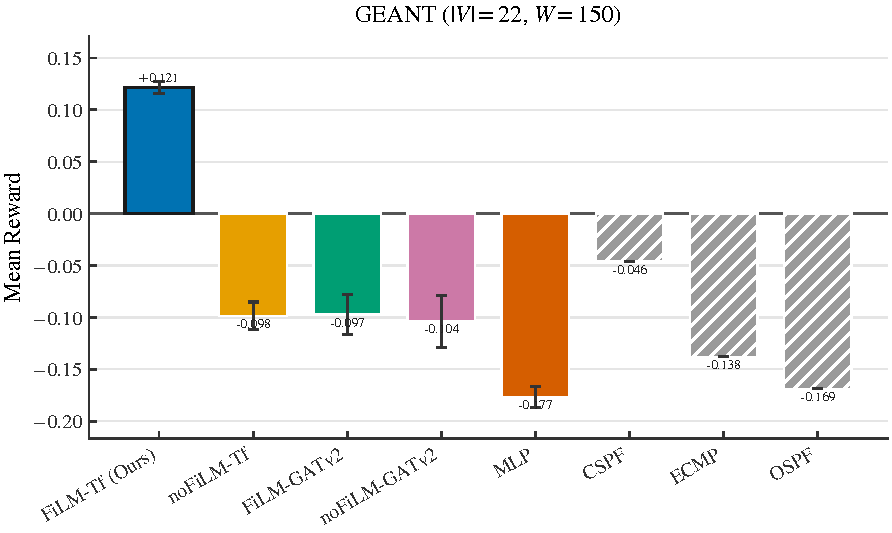
\includegraphics[width=0.32\textwidth]{p9b_bars_geant_linear_reward.pdf}\hfill
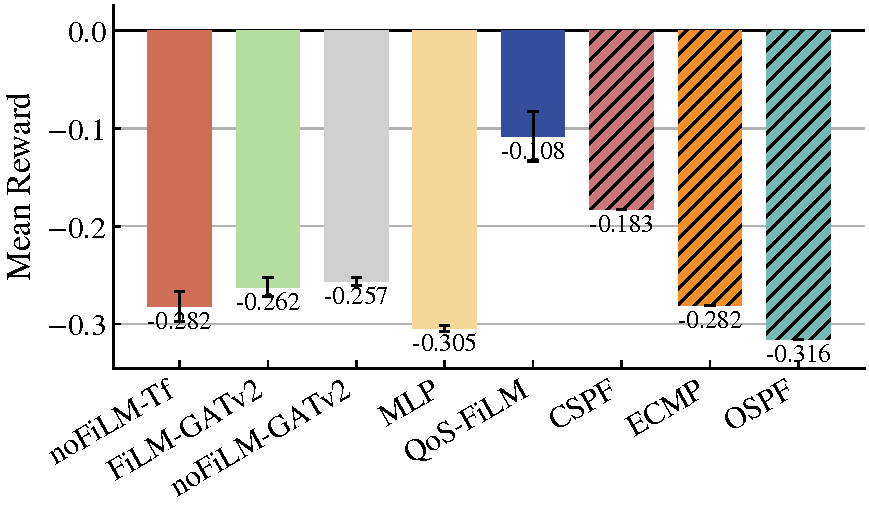
\includegraphics[width=0.32\textwidth]{p9b_bars_nobel_eu_reward.pdf}\hfill
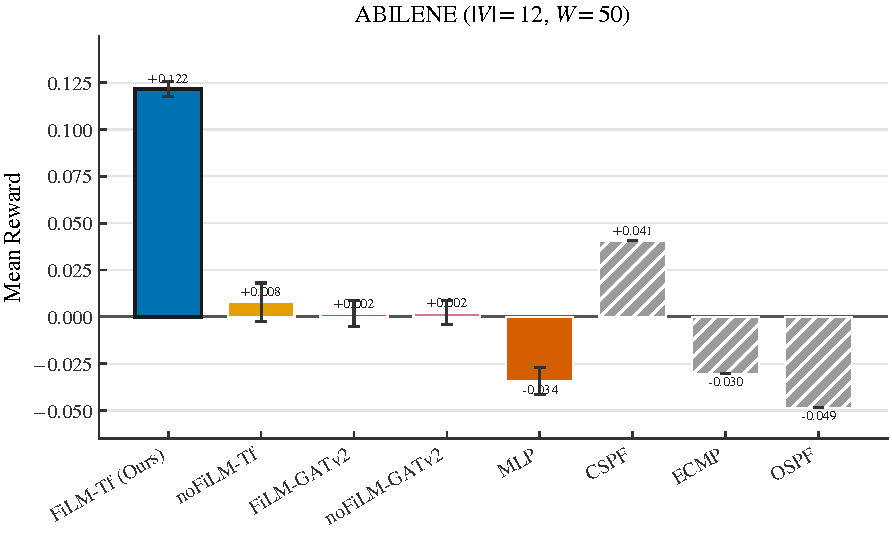
\includegraphics[width=0.32\textwidth]{p9b_bars_abilene_reward.pdf}\\[2pt]
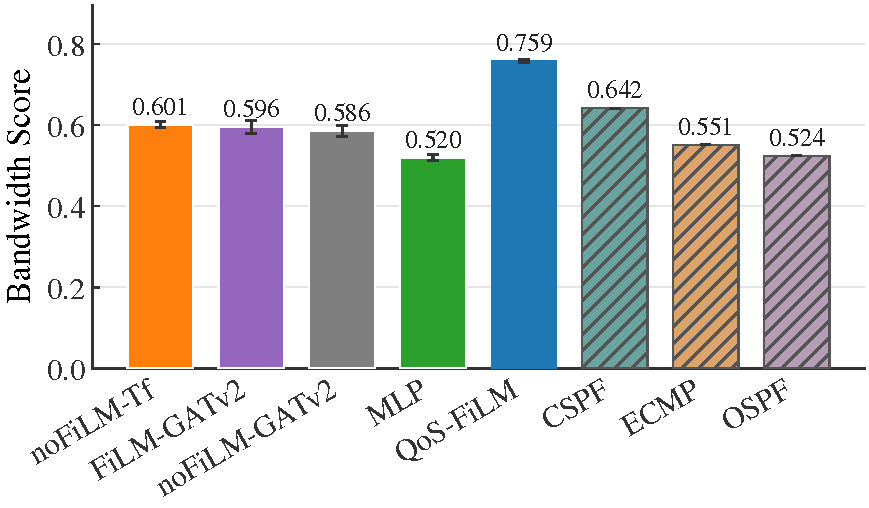
\includegraphics[width=0.32\textwidth]{p9b_bars_geant_linear_bw.pdf}\hfill
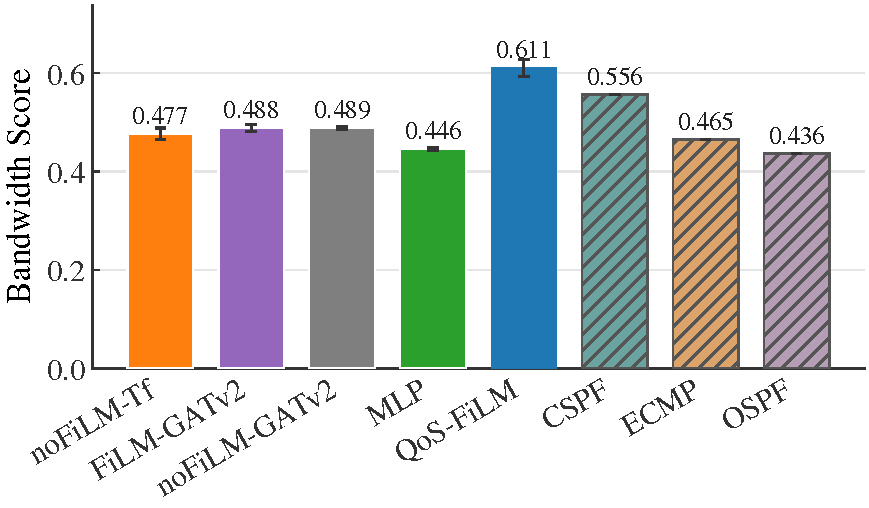
\includegraphics[width=0.32\textwidth]{p9b_bars_nobel_eu_bw.pdf}\hfill
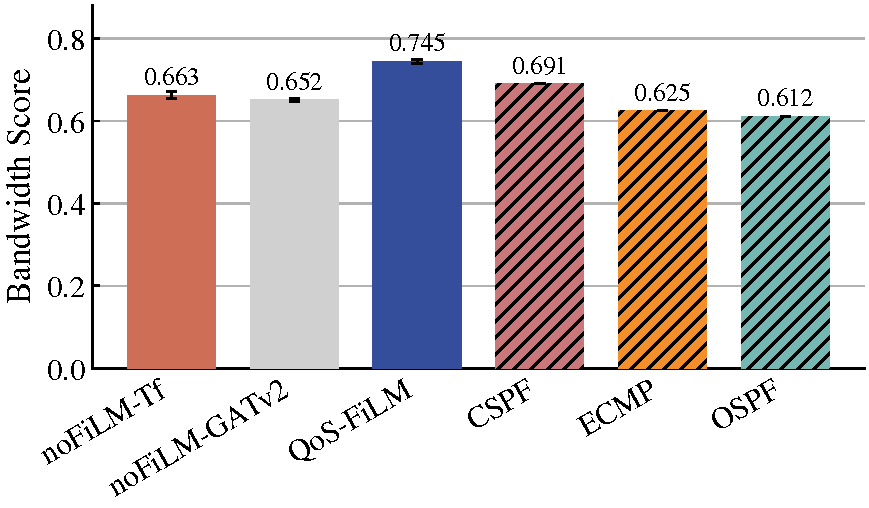
\includegraphics[width=0.32\textwidth]{p9b_bars_abilene_bw.pdf}\\[2pt]
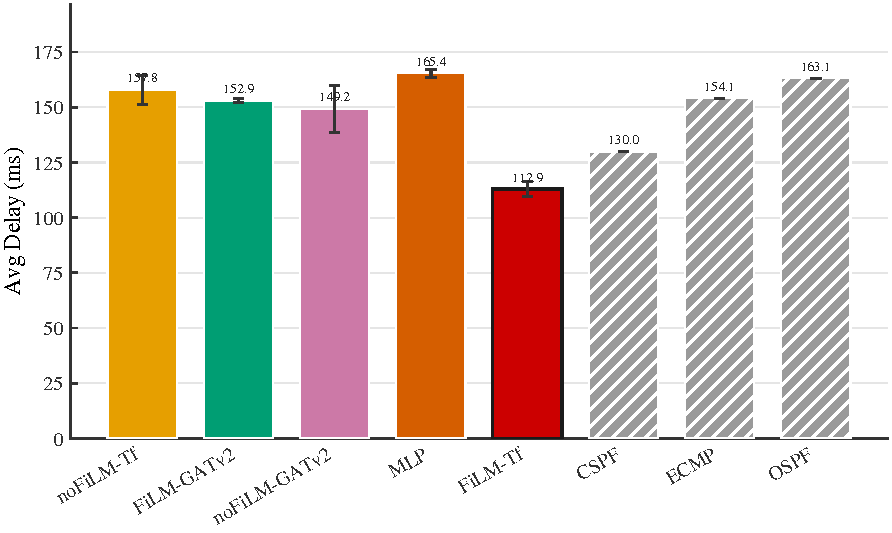
\includegraphics[width=0.32\textwidth]{p9b_bars_geant_linear_delay.pdf}\hfill
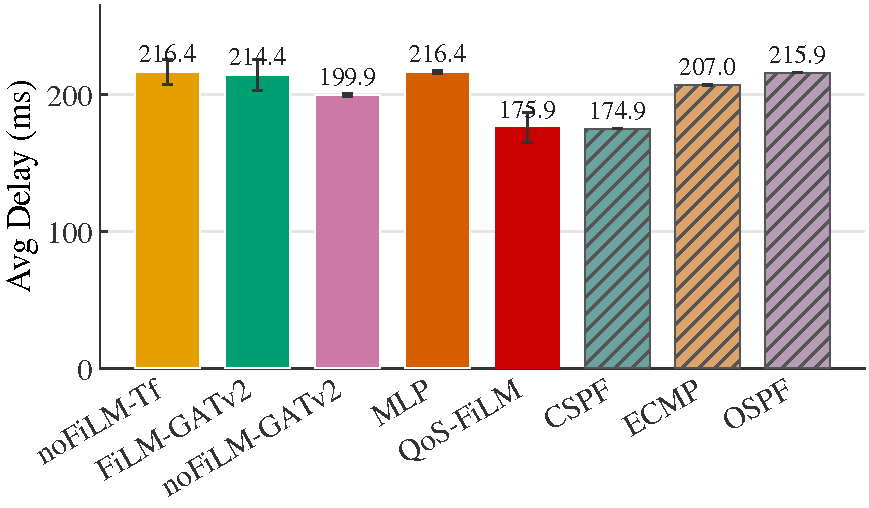
\includegraphics[width=0.32\textwidth]{p9b_bars_nobel_eu_delay.pdf}\hfill
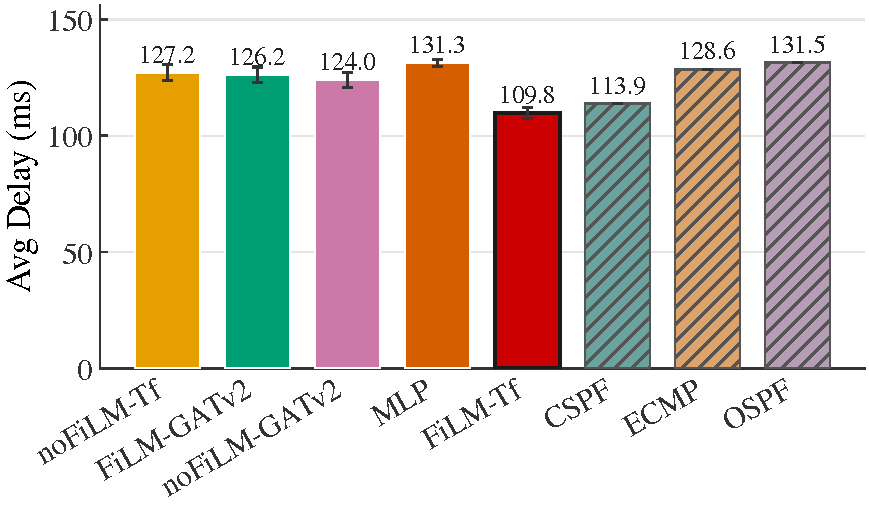
\includegraphics[width=0.32\textwidth]{p9b_bars_abilene_delay.pdf}
\caption{主线一：三个拓扑上的最终性能条形图对比。上行：平均奖励（3 种子均值，误差棒为 $\pm$标准差）；中行：带宽服务率；下行：平均时延（ms）。列从左到右：GEANT（$W\!=\!150$）、NOBEL-EU（$W\!=\!150$）、ABILENE（$W\!=\!50$）。彩色实心为学习型网络变体（QoS-FiLM 高亮），灰色斜纹为静态基线。}
\label{fig:main_bars}
\end{figure*}

\subsection{主线二：表示能力消融——消息传递与意图条件化}
\label{sec:exp:repr}

本节回答：是什么赋予了 QoS-FiLM超越经典算法的表示能力？为隔离 FiLM 条件化的贡献，我们沿"无图结构 $\to$ 有图结构但无流感知 $\to$ 有图结构且流感知"这一递进路径设计三个变体（图~\ref{fig:main_bars}），三者共享同一 TransformerConv 骨干与超参，仅表示机制不同：
\begin{itemize}
\item \textbf{MLP}（无消息传递）：移除消息传递，将式~\eqref{eq:conv} 的 $\mathrm{Conv}$ 替换为逐节点 MLP（仍保留 FiLM 调制），忽略边集 $E$ 与链路特征 $f$，用以检验图结构信息是否必要。
\item \textbf{noFiLM-Tf}（有消息传递但仅在末端拼接意图）：去掉式~\eqref{eq:film} 的 $\gamma,\beta$ 调制（等价于 $\gamma\equiv 0,\beta\equiv 0$），意图向量 $m_t$ 不进入消息传递、仅在末端打分器处与路径嵌入拼接，即所有流看到同一张图。
\item \textbf{QoS-FiLM}（逐层注入意图）：本文方法，在每一层都以式~\eqref{eq:film} 的 FiLM 仿射变换调制节点表示。
\end{itemize}

\textbf{消息传递是基础。} MLP 基线在三项指标上均最差（均值奖励 $-0.177$、BW Score $0.520$），且所有流退化为选同一路径槽（表~\ref{tab:film_w150_bw}中各类得分趋同，近 OSPF 等价行为）。没有邻居聚合，模型无法感知链路利用率的全局分布，也无法为不同意图的流差异化选路——这印证了图结构信息对路由学习的不可或缺。

\textbf{逐层注入意图（FiLM）带来显著增益。} 在相同的 GNN 骨干下，逐层注入流意图的 QoS-FiLM（$+0.121$）显著优于仅在末端拼接意图的 noFiLM-Tf（$-0.098$），$\Delta R\!=\!+0.219$；BW Score 提升 $+0.158$（$0.759$ vs $0.601$），平均时延从 $157.8$ 降至 $112.9$（降低 $44.9$ms）。图~\ref{fig:repr_training} 给出两种变体的 Eval Reward 训练曲线。noFiLM-Tf 的劣势源于意图信息仅在末端拼接、无法对逐层节点表示做 $\gamma\!\cdot\! x+\beta$ 调制，因而无法随流意图重塑消息传递过程。该趋势在三个拓扑上一致（图~\ref{fig:repr_training}）：QoS-FiLM均明显领先 noFiLM-Tf 与 MLP，且收敛更快、方差更小（NOBEL-EU 上 QoS-FiLM $-0.108$ vs noFiLM-Tf $-0.282$；ABILENE 上 $+0.122$ vs $+0.008$）。

\begin{figure*}[t]
\centering
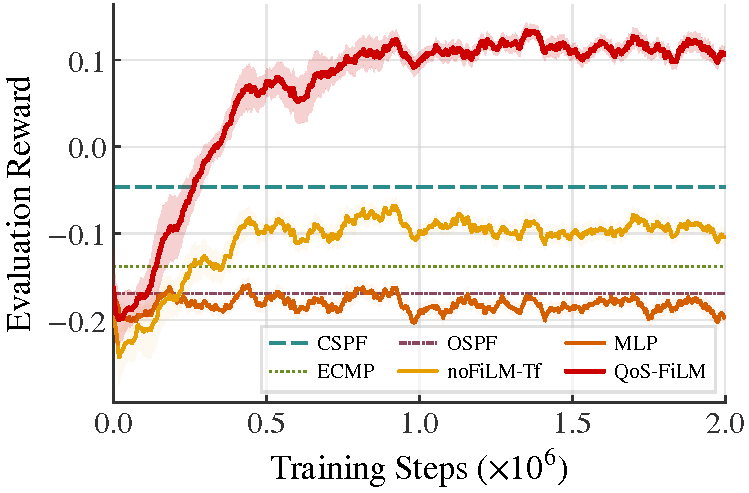
\includegraphics[width=0.32\textwidth]{p9b_groupA_geant_linear_eval.pdf}\hfill
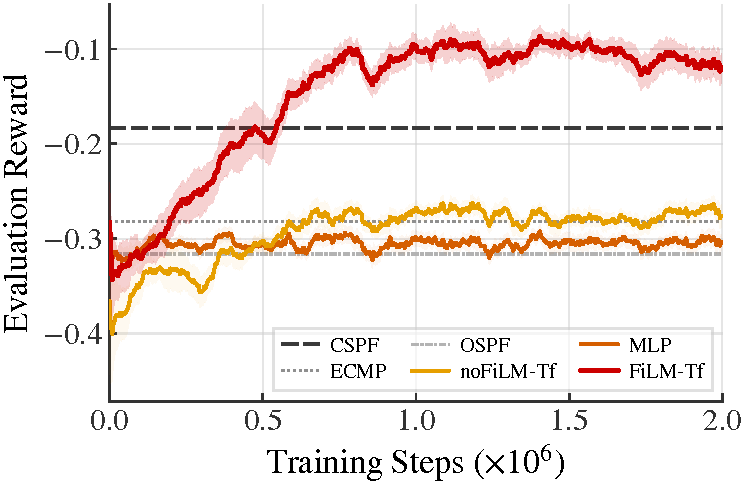
\includegraphics[width=0.32\textwidth]{p9b_groupA_nobel_eu_eval.pdf}\hfill
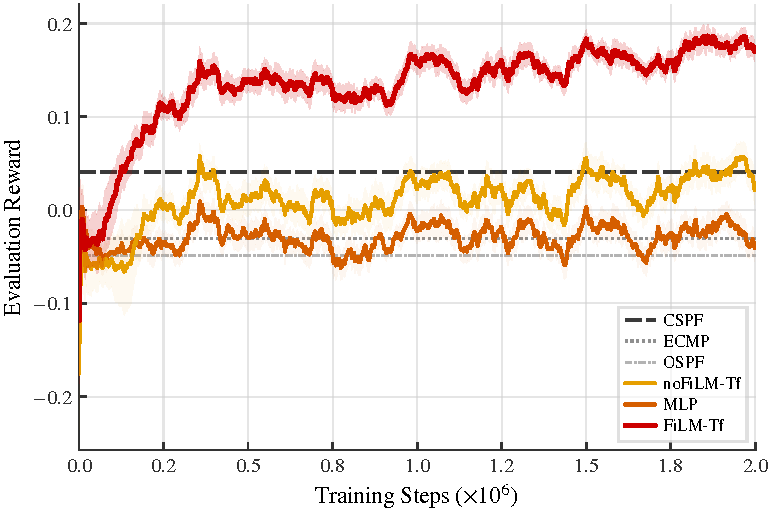
\includegraphics[width=0.32\textwidth]{p9b_groupA_abilene_eval.pdf}\\[2pt]
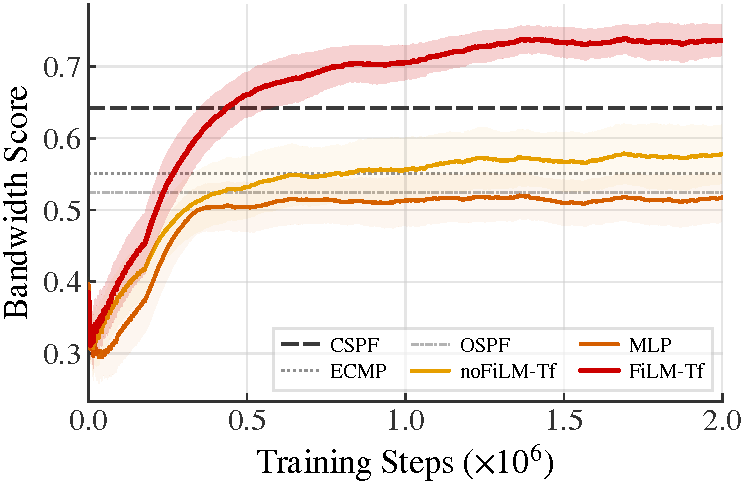
\includegraphics[width=0.32\textwidth]{p9b_groupA_geant_linear_bw.pdf}\hfill
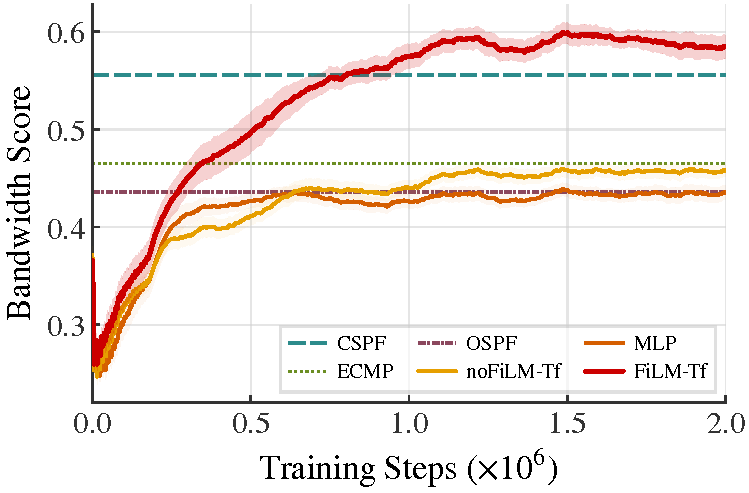
\includegraphics[width=0.32\textwidth]{p9b_groupA_nobel_eu_bw.pdf}\hfill
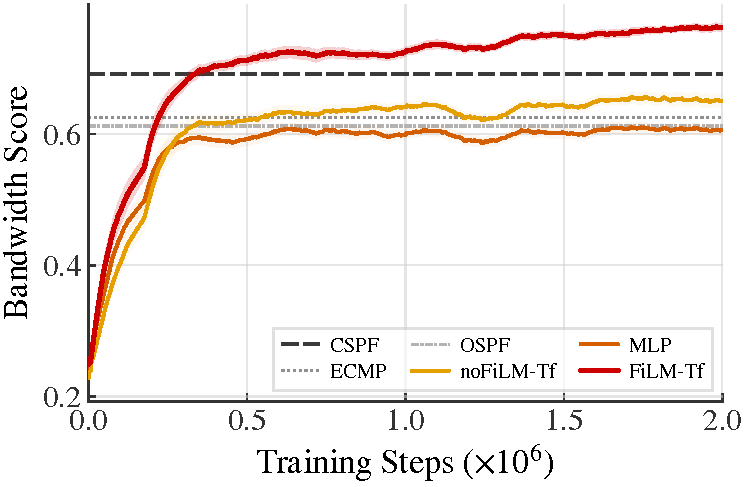
\includegraphics[width=0.32\textwidth]{p9b_groupA_abilene_bw.pdf}
\caption{主线二：QoS-FiLM、noFiLM-Tf 与 MLP 在三个拓扑上的训练曲线（3 种子均值$\pm$标准差置信带）。上行：Evaluation Reward；下行：Bandwidth Service Rate。列从左到右：GEANT（$W\!=\!150$）、NOBEL-EU（$W\!=\!150$）、ABILENE（$W\!=\!50$）。灰色虚线为经典基线的最终评估性能。}
\label{fig:repr_training}
\end{figure*}

按 $\phi$ 分桶来看（表~\ref{tab:film_w150_phi}），QoS-FiLM在时延敏感桶（$\phi<0.2$）的时延仅 $77.6$，较 noFiLM-Tf（$146.0$）降低 $68.4$ms；而在非时延敏感桶（$\phi\geq 0.8$）QoS-FiLM 的时延（$290.0$）反而高于 noFiLM-Tf（$225.9$）。这一"低降高升"模式正是 FiLM 条件化期望的行为：策略理解了不同 $\phi$ 的语义，主动将高意图流的时延资源分配给低意图流，以极低的代价换取了低意图桶服务质量的显著提升。按带宽类别（表~\ref{tab:film_w150_bw}），QoS-FiLM在 small 流上的 BW Score 达 $0.932$（noFiLM-Tf 仅 $0.669$，增益 $+0.263$），mid 流同样大幅领先（$0.857$ vs $0.614$）；big 流上 QoS-FiLM 略低（$0.348$ vs $0.483$），但以较小的 big 流代价换取了 small/mid 流的超高得分，整体权衡极为有利。

\begin{table}[t]
\centering
\caption{主线二消融——$\phi$ 分桶时延（$W\!=\!150$，200 ep × 3 seeds）\protect\footnotemark[1]。}
\label{tab:film_w150_phi}
\setlength{\tabcolsep}{3pt}
\begin{tabular}{lccc}
\toprule
模型 & $\phi<0.2$ & $0.2\!\le\!\phi\!<\!0.8$ & $\phi\!\ge\!0.8$ \\
\midrule
\textbf{QoS-FiLM} & $\mathbf{77.6}$ & $190.0$ & $290.0$ \\
noFiLM-Tf        & $146.0$ & $181.7$ & $225.9$ \\
MLP              & $156.3$ & $183.7$ & $220.2$ \\
\bottomrule
\end{tabular}
\end{table}

\begin{table}[t]
\centering
\caption{主线二消融——BW 类别（$W\!=\!150$，200 ep × 3 seeds）\protect\footnotemark[1]。}
\label{tab:film_w150_bw}
\setlength{\tabcolsep}{3pt}
\begin{tabular}{lccc}
\toprule
模型 & $b<8$ & $8\!\le\!b\!<\!32$ & $b\!\ge\!32$ \\
\midrule
\textbf{QoS-FiLM} & $\mathbf{0.932}$ & $\mathbf{0.857}$ & $0.348$ \\
noFiLM-Tf        & $0.669$ & $0.614$ & $0.483$ \\
MLP              & $0.568$ & $0.531$ & $0.431$ \\
\bottomrule
\end{tabular}
\end{table}
\footnotetext[1]{所有指标均为 GEANT 上 3 个随机种子的均值汇总（200 ep × 3 seeds，$W\!=\!150$）。}

\subsection{主线三：图注意力算子选择——TransformerConv vs GATv2Conv}
\label{sec:exp:conv}

本节回答：在相同的 FiLM 条件化框架下，底层图注意力算子的选择对性能有多大影响？TransformerConv 使用点积注意力~\cite{Shi2021_UniMP}，GATv2Conv 使用动态加性注意力~\cite{Brody2022_GATv2}，二者代表了两种不同的注意力范式。图~\ref{fig:conv_training} 给出三个拓扑上两种算子下 QoS-FiLM（以及作为参照的 noFiLM-GATv2）的训练曲线对比；可见 QoS-FiLM 在三个拓扑上均稳定领先 FiLM-GATv2。

\begin{figure*}[t]
\centering
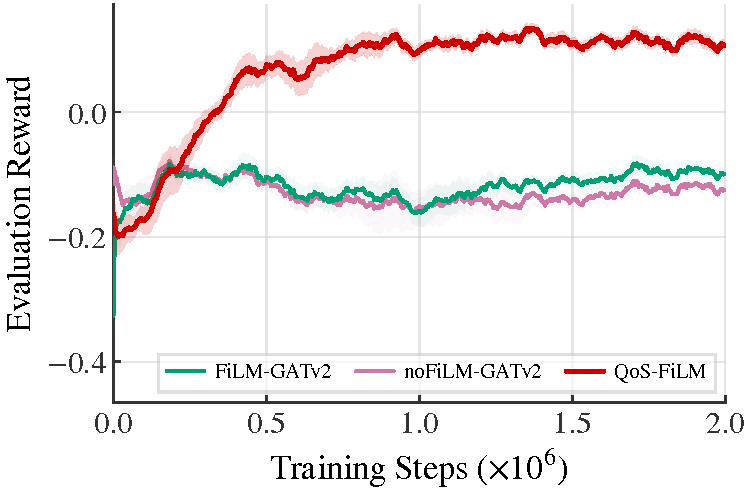
\includegraphics[width=0.32\textwidth]{p9b_groupB_geant_linear_eval.pdf}\hfill
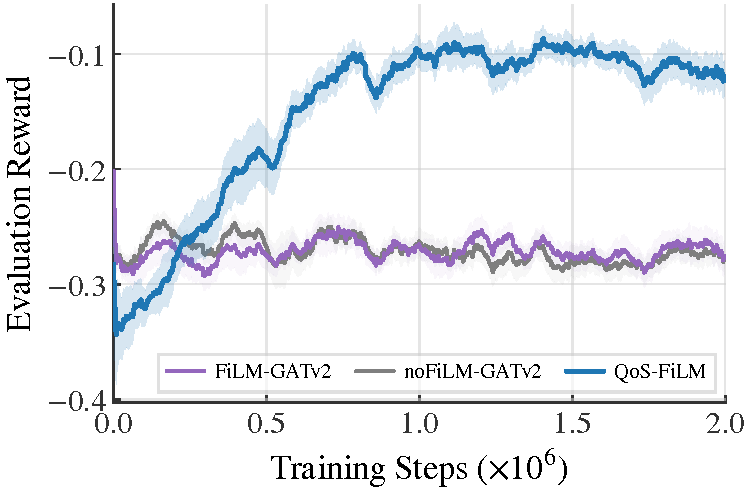
\includegraphics[width=0.32\textwidth]{p9b_groupB_nobel_eu_eval.pdf}\hfill
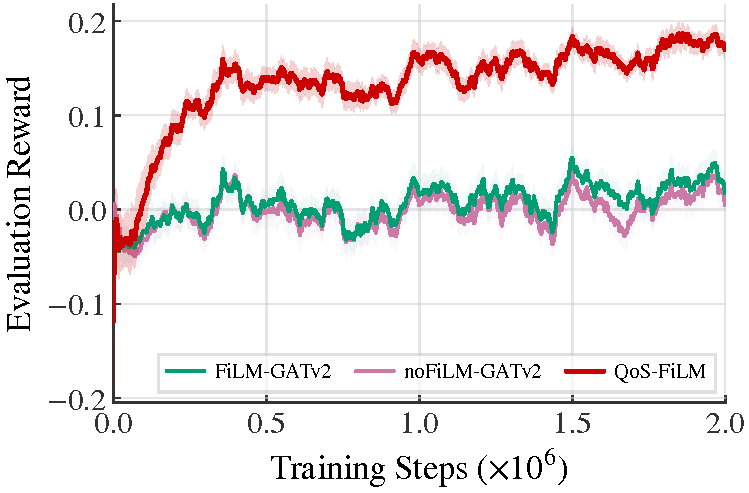
\includegraphics[width=0.32\textwidth]{p9b_groupB_abilene_eval.pdf}\\[2pt]
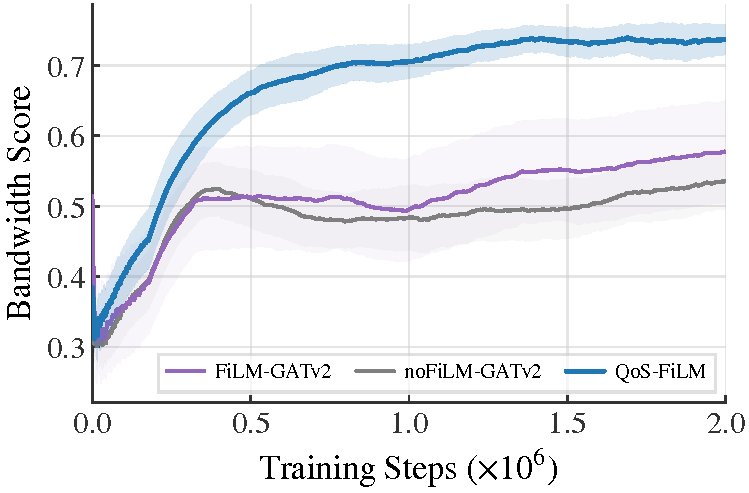
\includegraphics[width=0.32\textwidth]{p9b_groupB_geant_linear_bw.pdf}\hfill
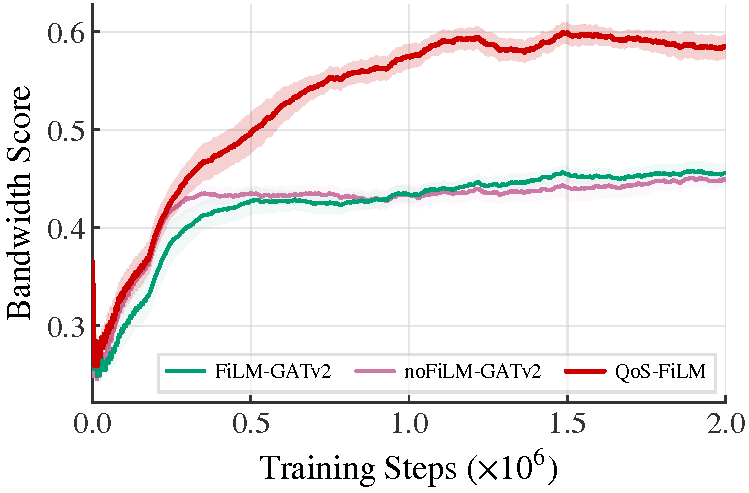
\includegraphics[width=0.32\textwidth]{p9b_groupB_nobel_eu_bw.pdf}\hfill
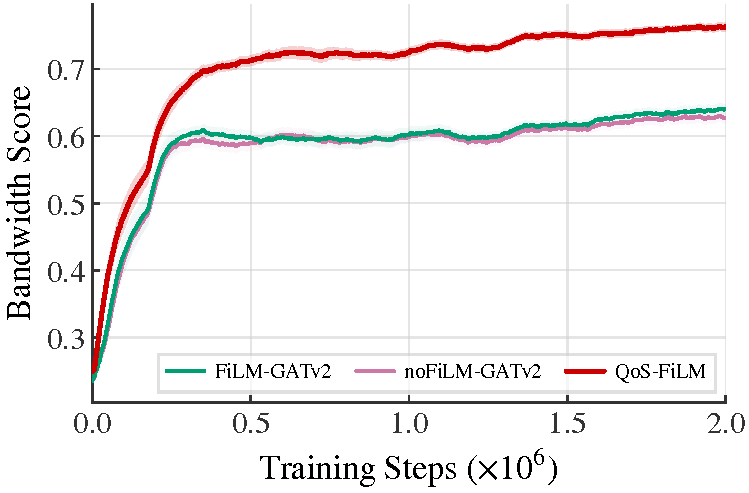
\includegraphics[width=0.32\textwidth]{p9b_groupB_abilene_bw.pdf}
\caption{主线三：QoS-FiLM、FiLM-GATv2 与 noFiLM-GATv2 在三个拓扑上的训练曲线（3 种子均值$\pm$标准差置信带）。上行：Evaluation Reward；下行：Bandwidth Service Rate。列从左到右：GEANT（$W\!=\!150$）、NOBEL-EU（$W\!=\!150$）、ABILENE（$W\!=\!50$）。}
\label{fig:conv_training}
\end{figure*}

从最终策略质量看（图~\ref{fig:conv_training}），QoS-FiLM（TransformerConv$+$FiLM）在平均奖励（$+0.121$）与带宽得分（$0.759$）上最优，大幅领先 FiLM-GATv2（$-0.097$，$0.596$），BW Score 差距 $+0.163$。两种算子性能差异的根源在于对链路属性（时延、容量、剩余带宽 $f_e=[d_e,c_e,b_e^{\text{res}}]$）的处理方式根本不同。TransformerConv~\cite{Shi2021_UniMP} 将链路属性同时注入注意力键与消息值：注意力权重 $\alpha_{i,j}=\mathrm{softmax}((\mathbf{W}_3\mathbf{x}_i)^{\top}(\mathbf{W}_4\mathbf{x}_j+\mathbf{W}_6\mathbf{e}_{ij})/\sqrt{d})$，消息 $\mathbf{W}_2\mathbf{x}_j+\mathbf{W}_6\mathbf{e}_{ij}$。链路特征 $\mathbf{e}_{ij}$ 通过乘性交互（内积）独立调节注意力——高剩余带宽的链路可以不依赖目标节点特征而获得更高注意力权重；同时链路特征直接构成消息内容，使聚合信息天然携带链路质量信号。相比之下，GATv2Conv~\cite{Brody2022_GATv2} 以加性方式混合链路与节点特征：$\alpha_{i,j}\propto\exp(\mathbf{a}^{\top}\mathrm{LeakyReLU}(\mathbf{\Theta}_s\mathbf{x}_i+\mathbf{\Theta}_t\mathbf{x}_j+\mathbf{\Theta}_e\mathbf{e}_{ij}))$。链路特征与源、目标节点特征经线性求和后共同进入非线性激活，导致链路质量信号与节点特征高度耦合——一条高带宽链路的注意力权重严重依赖于邻接节点表示，链路属性的独立判别力被稀释。在路由场景中，链路剩余带宽是路径选择的硬约束信号，应当独立、直接地影响邻居聚合；TransformerConv 的链路属性双通道注入（键+值）天然契合这一需求，而 GATv2Conv 的加性混合则削弱了链路质量的独立表达能力。

按 $\phi$ 分桶来看（表~\ref{tab:conv_w150_phi}），QoS-FiLM 同样呈现第~\ref{sec:exp:repr} 节所述的"低降高升"模式：低意图桶时延仅 $77.6$（GATv2 为 $135.2$，降低 $57.6$ms），高意图桶时延 $290.0$ 略高于 GATv2 的 $253.5$——TransformerConv 比 GATv2 更精准地识别了流的 $\phi$ 语义，将高意图流的时延资源让渡给低意图流。按带宽类别（表~\ref{tab:conv_w150_bw}），QoS-FiLM 的 small/mid 带宽得分（$0.932$/$0.857$）均大幅领先 FiLM-GATv2（$0.667$/$0.618$），big 流上略低（$0.348$ vs $0.456$），以较小的 big 流代价换取了 small/mid 流的超高得分。

\begin{table}[t]
\centering
\caption{主线三消融——$\phi$ 分桶时延（$W\!=\!150$，200 ep × 3 seeds）。}
\label{tab:conv_w150_phi}
\setlength{\tabcolsep}{3pt}
\begin{tabular}{lccc}

\toprule
模型 & $b<8$ & $8\!\le\!b\!<\!32$ & $b\!\ge\!32$ \\
\midrule
\textbf{QoS-FiLM} & $\mathbf{77.6}$ & $190.0$ & $290.0$ \\
FiLM-GATv2       & $135.2$ & $189.1$ & $253.5$ \\
MLP              & $156.3$ & $183.7$ & $220.2$ \\
\bottomrule

\end{tabular}
\end{table}

\begin{table}[t]
\centering
\caption{主线三消融——BW 类别（$W\!=\!150$，200 ep × 3 seeds）。}
\label{tab:conv_w150_bw}
\setlength{\tabcolsep}{3pt}
\begin{tabular}{lccc}
\toprule
模型 & small BW & mid BW & big BW \\
\midrule
\textbf{QoS-FiLM} & $\mathbf{0.932}$ & $\mathbf{0.857}$ & $0.348$ \\
FiLM-GATv2       & $0.667$ & $0.618$ & $0.456$ \\
MLP              & $0.568$ & $0.531$ & $0.431$ \\
\bottomrule
\end{tabular}
\end{table}

\subsubsection{FiLM 与算子的强协同：二维不可加}
\label{sec:exp:synergy}

本节回答算子选择（TransformerConv vs GATv2）与条件化机制（FiLM vs noFiLM）是各自独立贡献，还是存在交互？为此我们补齐 noFiLM-GATv2 变体，构成算子$\times$条件化的 $2\times2$ 对比表（表~\ref{tab:synergy_2x2}）。

关键发现是：\emph{FiLM 的增益强烈依赖于底层算子}。在 TransformerConv 上，引入 FiLM 带来 $\Delta R\!=\!+0.219$（$-0.098\!\to\!+0.121$）的巨大提升；但在 GATv2 上，FiLM 的增益仅 $\Delta R\!=\!+0.007$（$-0.104\!\to\!-0.097$），几乎失效。这表明两个维度并非独立可加，而是存在强协同：上述链路属性处理方式的差异放大了 FiLM 效果的差距——TransformerConv 将链路属性独立注入注意力键与消息值，为 FiLM 逐层意图调制提供了高质量、链路级可区分的表示基础；而 GATv2Conv 将链路属性混入节点特征，即使 FiLM 在每层准确注入了流意图，意图信号也难以通过已被稀释的链路质量表示转化为有效的路径区分。因此，TransformerConv $+$ FiLM 的组合并非两个独立优势的简单叠加，而是二者缺一不可的协同产物。

\begin{table}[t]
\centering
\caption{算子$\times$条件化的 $2\times2$ 对比表（Mean $R$，$W\!=\!150$，200 ep × 3 seeds）。括号内为同一算子上 FiLM 带来的增益 $\Delta R$。}
\label{tab:synergy_2x2}
\setlength{\tabcolsep}{6pt}
\begin{tabular}{lcc}
\toprule
 & TransformerConv & GATv2Conv \\
\midrule
$+$FiLM & $\mathbf{+0.121}$ & $-0.097$ \\
$-$FiLM & $-0.098$ & $-0.104$ \\
\midrule
$\Delta R$ (FiLM 增益) & $\mathbf{+0.219}$ & $+0.007$ \\
\bottomrule
\end{tabular}
\end{table}

值得强调的是，FiLM 的参数开销是一个与算子无关的常数 $+6{,}144$（相对开销仅 $+0.6\%\sim+2.0\%$，来自 $\mathrm{MLP}_\gamma,\mathrm{MLP}_\beta$ 两个意图$\to$隐藏维的线性层）。因此在 TransformerConv 骨干上，FiLM 以不足 $1\%$ 的参数换取了 $\Delta R\!=\!+0.219$ 的显著提升，性价比极高。


\subsection{主线四：可解释性——流意图如何影响表示与决策}
\label{sec:exp:interp}

为进一步理解 FiLM 条件化的作用机制，本节从\emph{表示层}与\emph{决策层}两个角度，考察 FiLM 与 noFiLM-Tf 在响应流意图时的本质差异。

\textbf{表示层：意图驱动的隐藏特征敏感性。} 固定网络拓扑与链路利用率状态，对相同的 (src, dst) 节点对注入 QoS 意图 $\phi$ 逐渐变化的流，观察 Encoder 映射出的隐藏特征。我们在 $8$ 个随机网络状态、$\phi\!\in\!\{0.05,0.2,0.5,0.8,0.95\}$ 上统计意图敏感性（相同状态下 $\phi$ 变化引起的隐藏表示总变化量）：FiLM 编码器的敏感性高达 $46.46$，而 noFiLM-Tf 仅为 $1.4\times10^{-6}$（数值零），二者相差七个数量级（表~\ref{tab:interp_repr}）。更进一步，随着 $\phi$ 从基准逐渐增大（$0.05\!\to\!0.95$），FiLM 表示的漂移量单调增大（$0\!\to\!8.6\!\to\!25.8\!\to\!40.5\!\to\!46.5$），说明意图被平滑、连续地编码进节点表示；而 noFiLM-Tf 的漂移量始终为零。这从架构层面严格验证了消融设计（noFiLM 确实看不到意图），也是 FiLM 将逐流意图注入节点表示的直接量化证据。图~\ref{fig:embedding_separation} 进一步给出两种编码器隐藏特征的 PCA 投影：FiLM 的表示随 $\phi$ 连续迁移，noFiLM-Tf 的表示则完全重叠。

\begin{table}[t]
\centering
\caption{主线四表示层：相同网络状态、仅 $\phi$ 变化时的隐藏表示变化（GEANT，$8$ 状态均值）。}
\label{tab:interp_repr}
\setlength{\tabcolsep}{5pt}
\begin{tabular}{lcc}
\toprule
 & 意图敏感性 & 漂移量（$\phi\!:0.05\!\to\!0.95$） \\
\midrule
\textbf{QoS-FiLM}  & $\mathbf{46.46}$ & $0\to8.6\to25.8\to40.5\to46.5$ \\
noFiLM-Tf         & $1.4\times10^{-6}$ & 全零 \\
\bottomrule
\end{tabular}
\end{table}

\begin{figure*}[t]
\centering
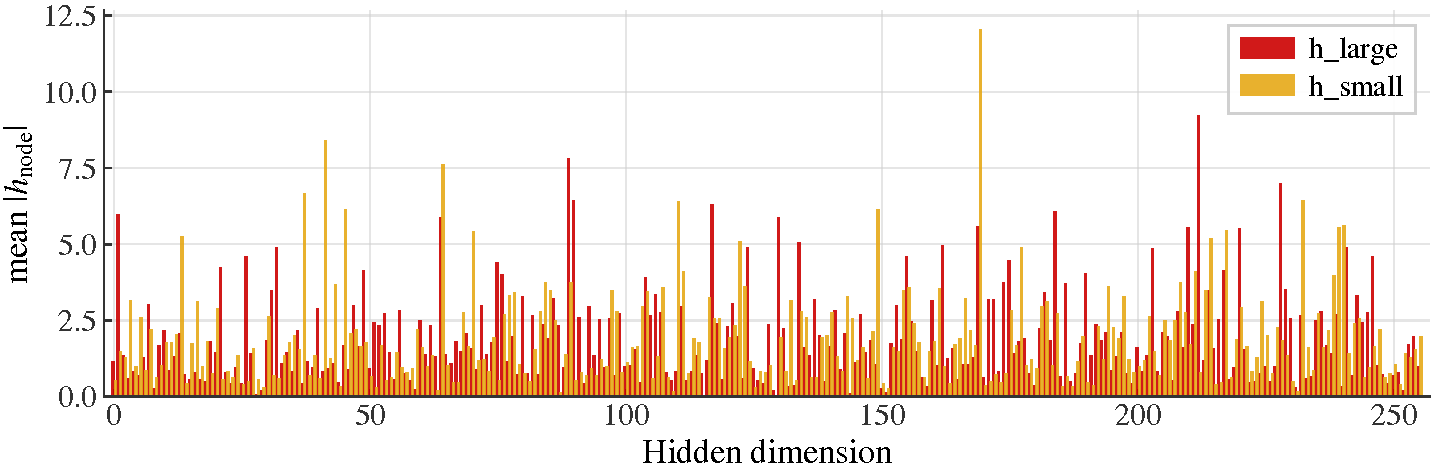
\includegraphics[width=0.48\textwidth]{p9b_hidden_diff_film_tf.pdf}\hfill
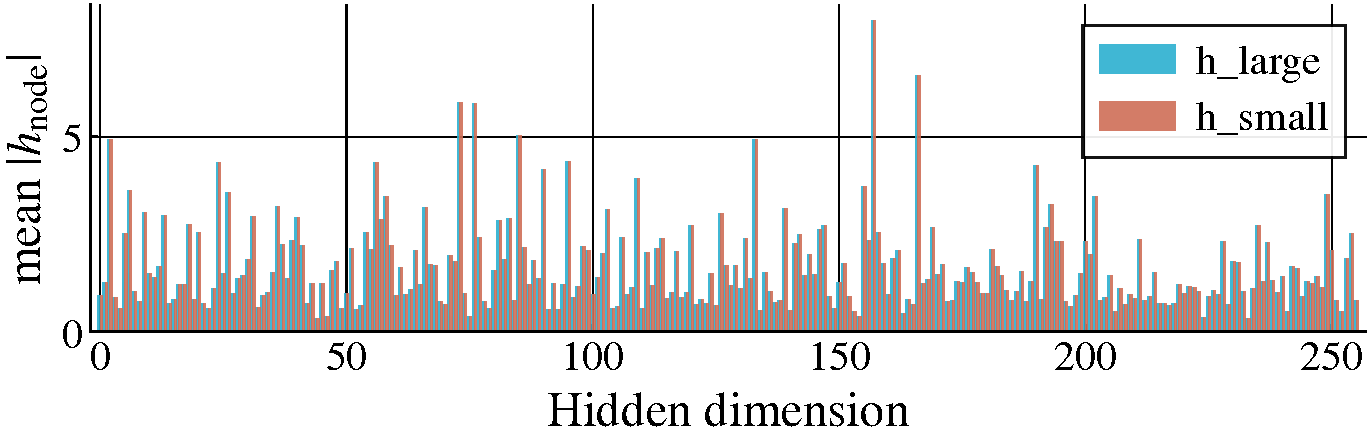
\includegraphics[width=0.48\textwidth]{p9b_hidden_diff_nofilm_tf.pdf}
\caption{相同网络状态与 (src, dst) 对下，极端小流与极端大流的隐藏特征对比（左：QoS-FiLM；右：noFiLM-Tf）。}
\label{fig:embedding_separation}
\end{figure*}

\textbf{决策层：意图驱动的路径选择多样性。} 表示层的差异最终体现为选路行为的变化。我们在 $200$ 个测试 episode、共 $460$ 个 (src, dst) 对上统计两个变体的路径槽选择分布的熵（以 bits 计，越高说明选择越多样化、越依状态和意图差异化）。FiLM 的平均熵为 $2.235$，显著高于 noFiLM-Tf 的 $1.962$（配对 $t\!\approx\!14.7$，极显著）；在 $76\%$ 的 (src, dst) 对上 FiLM 的熵更高，FiLM 平均启用 $10.4$ 个路径槽而 noFiLM-Tf 仅 $7.9$ 个。这表明 FiLM 策略能根据当前链路状态与每条流的意图做出更细腻、更差异化的路径选择，而 noFiLM-Tf 因看不到意图、只能依赖状态，选择更集中于少数路径槽。这一对比与表示层的敏感性证据相互印证：\emph{意图被 FiLM 注入表示（表示层）$\to$ 驱动更多样化的路径选择（决策层）}，构成了从意图到决策的完整因果链。


\section{Conclusion}
\label{sec:conclusion}
本文提出 QoS-FiLM，一种以逐流 QoS 意图为条件信号的图神经网络架构，用于解决异构流量共存的在线路由问题。QoS-FiLM 通过特征级线性调制将流意图注入 GNN 的各层消息传递，使同一物理拓扑对不同 QoS 需求的流产生差异化的节点嵌入，从而消解 ``同图同嵌入'' 的表示同质化。实验表明，QoS-FiLM 在多个骨干网拓扑上的累积效用、带宽满足比和端到端时延均优于经典基线。消融研究证实逐层 FiLM 条件化较无流感知带来 $+0.219$ 的性能增益，可解释性分析验证了 FiLM 编码器对 QoS 意图具有极高的表示敏感性，而无流感知的对照组几乎无法感知意图变化。未来我们将围绕……

\bibliographystyle{IEEEtran}
\bibliography{related_work}

\end{document}
流感知图神经网络 — 会议论文依赖: ctex (中文), IEEEtran 文档类conference%
  {../experiments/p4_calibration/figures/pdf/}%
  {../experiments/p6_interpretability/figures/pdf/}%
  
% IEEEtran 下中文标题/作者按会议结构，本轮：问题定义 / 方法（含MDP建模）/ 实验% % 